% begin module improper-integral-type2-ex5
\begin{frame}
\begin{example}[Example 5, p. 548]
Find $\int_2^5 \frac{1}{\sqrt{x-2}}\diff x$.

\uncover<2->{Observe that $x = 2$ is a vertical asymptote for the integrand.}
\begin{columns}[c]
\column{.4\textwidth}
\ 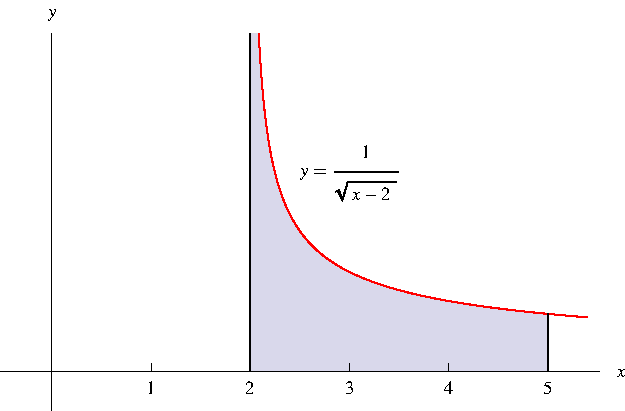
\includegraphics[height=4cm]{improper-integrals/pictures/08-08-ex5.pdf}%

\uncover<7->{Area = $2\sqrt{3}$}
\column{.6\textwidth}
\begin{eqnarray*}
& & %
\uncover<3->{%
\int_2^5 \frac{1}{\sqrt{x-2}}\diff x%
}\\%
& \uncover<3->{ = } &%
\uncover<3->{%
\lim_{t\rightarrow 2^+}\int_t^5 \frac{1}{\sqrt{x-2}}\diff x%
}\\%
& \uncover<4->{ = } &%
\uncover<4->{%
\lim_{t\rightarrow 2^+}\left[ 2\sqrt{x-2}\right]_t^5%
}\\%
& \uncover<5->{ = } &%
\uncover<5->{%
\lim_{t\rightarrow 2^+} 2(\sqrt{5-2} - \sqrt{t-2})%
}\\%
& \uncover<6->{ = } &%
\uncover<6->{%
2\sqrt{3}%
}\\%
\end{eqnarray*}
\end{columns}
\end{example}
\end{frame}
% end module improper-integral-type2-ex5
